\documentclass[12pt]{article}
\usepackage[top=1.5 in, bottom = 1.5 in, left = 1 in, right=1 in]{geometry}
\usepackage[american]{babel}
\usepackage[numbers]{natbib}
\usepackage{etoolbox}
\apptocmd{\thebibliography}{\raggedright}{}{}
\usepackage{amsmath}
\usepackage{amssymb, amsfonts, textcomp}
\usepackage{titlesec}
\usepackage{color}
\usepackage{multicol}
\usepackage{multirow}
\usepackage{tabu}
\usepackage{booktabs}
\usepackage{array}
\usepackage{hhline}
\usepackage{hyperref}
\usepackage{fontspec}
\setmainfont{Chaparral Pro}
\setromanfont{Chaparral Pro}
\setmonofont{Consolas}
\setsansfont{Myriad Pro}
\setcounter{secnumdepth}{5}
\pagestyle{plain}
\addto\captionsamerican{ %babel
	\renewcommand\contentsname{}
}

%\titleformat{<command>}[<shape>]{<format>}{<label>}{<sep>}{<before-code>}[<after-code>]
\titleformat{\subparagraph}[hang]
{\normalfont\normalsize\bfseries}{\thesubparagraph}{1 em}{}[]
%\titlespacing*{<command>}{<left>}{<before-sep>}{<after-sep>}
\titlespacing*{\subparagraph}{0 pt}{2 ex}{.25 ex}

\titleformat{\paragraph}[hang]
{\normalfont\normalsize\bfseries}{\theparagraph}{1 em}{}[]
\titlespacing*{\paragraph}{0 pt}{2 ex}{.25 ex}

\begin{document}
	\pagenumbering{gobble}
	\vspace*{2.8 in}
	\begin{huge}
		\begin{center}
			Software Requirements Specification
			\par
			for
			\par
			The Walking Game
			\par
		\end{center}
	\end{huge}
	\vspace*{2.5 in}
	\begin{large}
		\begin{flushright}
			Star Team
			
			Version: 1.0
			
			Date: 10/31/2014
		\end{flushright}
	\end{large}
	
	\clearpage
	\section*{Revision History}
	\begin{flushleft}
		\begin{tabular}{|p{0.14\linewidth}|p{0.12\linewidth}|p{0.45\linewidth}|p{0.18\linewidth}|}
			\hline
			\textbf{Revision \#} & \textbf{Date} & \textbf{Description} & \textbf{Author} \\\hline
			1.0 & 10/31/2014 & Initial revision & Samuel I. Gunadi \\\hline
		\end{tabular}
	\end{flushleft}
	\clearpage
	
	\clearpage
	\clearpage
	\setcounter{page}{0}
	
	\pagenumbering{arabic}
	\section{Introduction}
	The members of Star team are Samuel I. Gunadi, Roberto J. Kondurura, and Ryan Elegant. Star team has a goal to fulfill the requirements of the software engineering course at Universitas Pelita Harapan. The project website can be found at \begin{footnotesize}\url{https://github.com/samuelgunadi/thewalkinggame}\end{footnotesize}.
	
	\subsection{Purpose}
	This specification establishes the functional, performance, and development requirements for The Walking Game project. This document is intended to aid by Star Team in the development process and also by 
	
	\subsection{Scope}
	The project will have a Wavefront OBJ file parser; people 3D models, textures, and walking animations; textures with alpha blending; a textured floor; collision detection; simple command interpreter and scripting; nameplates; and an MMORPG style third-person camera. 
	
	The animation technique used in The Walking Games will not be skeletal animation; instead, it will be by loading one .obj for every key frame.
	
	This project aims to educate and entertain users---educate, by studying the source code, and entertain, by playing and interacting through the console. This project will mostly benefits the team as part of their Computer Graphics and Software Engineering course assignments.
	
	\subsection{Definitions, acronyms, and abbreviations}
	\vspace{0.1in}\noindent SRS --- Software Requirements Specification
	
	\vspace{0.1in}\noindent OpenGL --- Open Graphics Library
	
	\vspace{0.1in}\noindent OBJ --- Wavefront OBJ File Format
	
	\vspace{0.1in}\noindent GLEW --- The OpenGL Extension Wrangler Library 
	
	\vspace{0.1in}\noindent PDF --- Portable Document Format
	
	\vspace{0.1in}\noindent IDE --- Integrated Development Environment
	
	\vspace{0.1in}\noindent MMORPG --- Massively Multiplayer Online Role-Playing Game
	
	\nocite{*}
	
	\begingroup
	\subsection{References}
	\renewcommand{\section}[2]{}%
	\bibliographystyle{IEEEtranN}
	\bibliography{references}
	\endgroup
	
	\subsection{Overview}
	Section 1 identifies the scope of this document, the purpose of this document, lists the definitions, acronyms and references, and explains how the SRS is organized. Section 2 describes the general factors that affect the product and its requirements. This section does not state specific requirements. Instead, it provides a background for those requirements, which are defined in detail in Section 3 of the SRS, and makes them easier to understand. Section 3 contains all of the software requirements to a level of detail sufficient to enable designers to design a system to satisfy those requirements, and testers to test that the system satisfies those requirements.
	
	\clearpage
	\section{Overall description}
	
	\subsection{Product perspective}	
	
	\subsubsection{User interfaces}
	The Walking Game includes an interface resembling a RPG game with a console to provide additional functionalities and aid in testing and debugging process.
	
	\subsubsection{Hardware interfaces}
	The Walking Game should run on any computer hardware meeting the following criteria:
	\begin{itemize}
		\item Dual-core CPU
		\item OpenGL 4.3 compatible GPU with 2 GB memory
		\item 2 GB free hard disk space.
		\item Mouse with 3 buttons
		\item Keyboard with US layout
		\item 2 GB of RAM
	\end{itemize}
	
	\subsubsection{Software interfaces}
	The Walking Game integrates several external software to provide functionality:
	\begin{enumerate}
		\item GLFW. GLFW is used for creating windows with OpenGL contexts and receiving input and events. GLFW is multi-platform and supports Windows, OS X and many Unix-like systems. GLFW is licensed under the zlib/libpng license.
		\item GLEW. GLEW is a cross-platform open-source C/C++ extension loading library. GLEW provides efficient run-time mechanisms for determining which OpenGL extensions are supported on the target platform. OpenGL core and extension functionality is exposed in a single header file. GLEW has been tested on a variety of operating systems, including Windows, Linux, Mac OS X, FreeBSD, Irix, and Solaris.
		\item GLM. GLM is a header only C++ mathematics library for graphics software based on the OpenGL Shading Language (GLSL) specification and released under the MIT license.
	\end{enumerate}
	
	\subsection{Product functions}
	These are the main functional areas:
	
	\begin{itemize}
		\item \textbf{OBJ file parser.} OBJ files are generated by content creation tools and then parsed and loaded into GPU memory.
		
		\item \textbf{Texture loader.} Image files are generated by content creation tools and then parsed and loaded into GPU memory.
		
		\item \textbf{Character management.} The scene includes characters that are rendered with animations, textures, and geometry data, then the characters are labeled with nameplates and animated.
		
		\item \textbf{Command interpreter.} The console commands are inputted through the console and appropriate actions are executed.
		
		\item \textbf{Third-person camera.} The camera enables the user to view the scenes.
	\end{itemize}
	
	\subsection{User characteristics}
	No special knowledge or skills should be assumed on the part of the users. Although the user is expected to have experience in C/C++ to interact with the console. 
	
	\subsection{Constraints}
	The Walking Game may experience hardware limitations constrain for graphics requirements if installed in an incompatible computer.
	
	\subsection{Assumptions and Dependencies}
	The Walking Game is written with portability in mind and should run on Windows, OS X, and Linux.
	
	\clearpage
	
	\section{Specific requirements}
	\subsection{External interface requirements}
	\subsubsection{User interfaces}
	All interaction with the user is done via console and main window.
	
	\subsubsection{Hardware Interfaces}
	User interacts using computer display, mouse, and keyboard.
	
	\subsubsection{Software interfaces}
	The system should be capable of running on Windows, OS X, and Linux.
	
	\subsection{Classes}
	
	\subsubsection{Character}
	This class shall render a character and update its animation when it's walking.
	
	\subsubsection{Nameplate}
	This class shall label a character and render a text above the character.
	
	\subsubsection{Texture}
	This class shall aid managing textures.
	
	\subsubsection{Mesh}
	This class shall be capable of importing OBJ and uploading the geometrical data into the GPU. This class should be able to export and import the geometrical data into binary format to speed up the loading process.
	
	\subsubsection{Plane}
	This class shall represent a geometric plane.
	
	\subsubsection{Floor}
	This class shall render a textured plane.
	
	\subsubsection{Frustum}
	This class shall represent a frustum used by the camera.
	
	\subsubsection{Camera}
	This class shall provide camera functionalities to a scene.
	
	\subsubsection{Third-person camera}
	This class shall add the camera functionalities to follow a character.
	
	\subsubsection{Scene}
	This class shall abstract the scene.
	
	\subsubsection{Main scene}
	This class shall encapsulate the objects to be rendered.
	
	\subsubsection{Main event handler}
	This class shall handle keyboard and mouse inputs from user.
	
	\subsubsection{Shader program}
	This class shall encapsulate an OpenGL shader program.
	
	\subsubsection{Light}
	This class shall represent a light.
	
	\subsubsection{Material}
	This class shall represent a Phong shader material.
	
	\subsubsection{Thread pool}
	This class shall enable asynchronous tasks to be executed concurrently.
	
	\subsection{Performance requirements}
	No performance requirements have been specified by the clients.
	
	\subsection{Design constraints}
	No design constraints have been identified.
	
	\subsection{Software system attributes}
	\subsubsection{Reliability}
	\begin{enumerate}
		\item system should handle errors when processing console commands.
		\item The system should not crash during initialization and running.
	\end{enumerate}
	
	\subsubsection{Availability}
	\begin{enumerate}
		\item The system should recover corrupt files.
	\end{enumerate}
	
	\subsubsection{Security}
	\begin{enumerate}
		\item The system should provide logs to identify errors.
	\end{enumerate}
	
	\subsection{Other requirements}
	No other requirements have been identified.
	
	\clearpage
	\section{Supporting information}
	\subsection{Table of contents}
	\vspace{-0.5 in}
	\tableofcontents
	\subsection{Appendix A: Class diagram}
	\newgeometry{top=0 in, bottom = 0 in, left = 0 in, right = 0 in}
	\begin{figure}[t]
		\centering
		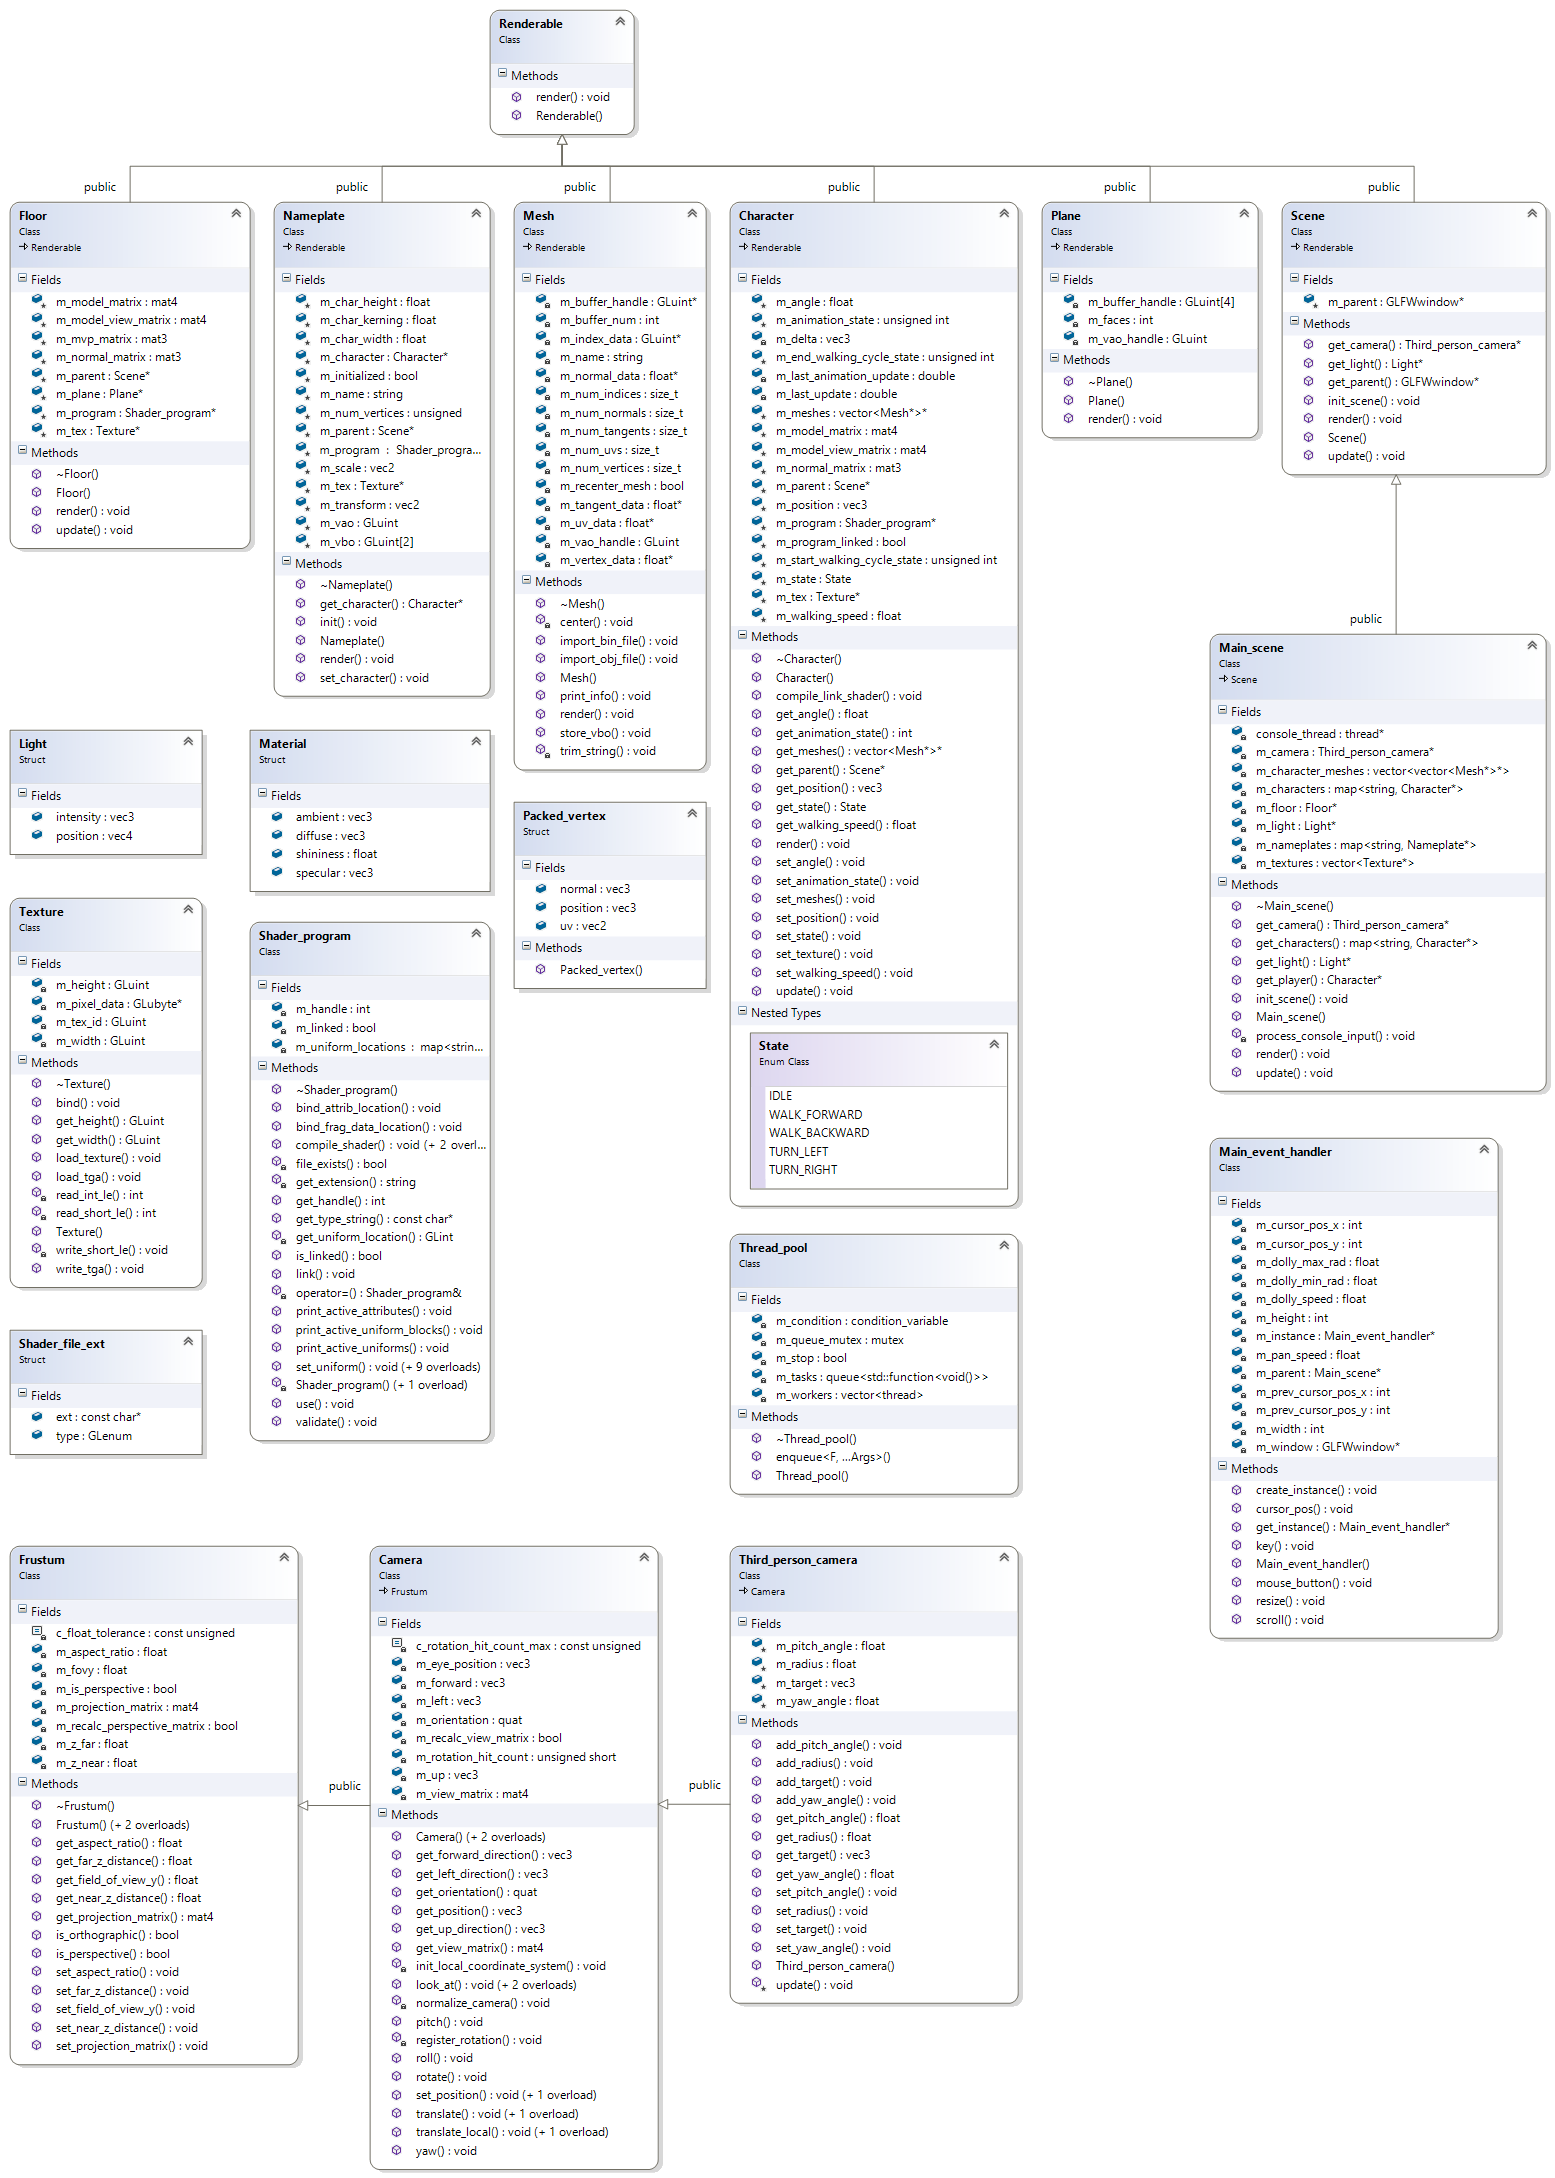
\includegraphics[width=\paperwidth, height=\paperheight]{class_diagram}
		\caption{}
		\label{fig:class_diagram}
	\end{figure}
	\restoregeometry
	
\end{document}